\chapter{Rozpoznawanie akordów muzycznych} \label{chapter:methodology}

% model (model.py), trening nadzorowany z ewaluacją (training.py, evaluate.py), trening
% nienadzorowany (mae_training.py)

% wstęp - model
Rozpoznawanie akordów muzycznych zostało zrealizowane za pomocą sieci neuronowych. Wykorzystana została popularna ostatnio w wielu obszarach architektura transformera \cite{vaswani_attention_2017}. Modele tego typu były wykorzystywane w najnowszych pracach związanych z rozpoznawaniem akordów, w tym w pracy \cite{park_bi-directional_2019} stanowiącej główny punkt odniesienie dla niniejszych badań.

% wstęp - metoda: self-supervised -> supervised
Zaproponowany sposób nauczenia sieci neuronowej zadania rozpoznawania akordów składa się z dwóch części: nienadzorowanego treningu wstępnego i nadzorowanego treningu właściwego. W praktyce sam trening nadzorowany, czyli oparty o oznaczone wcześniej przykłady uczące (pary nagrań muzycznych i plików z symbolami akordów), pozwala nauczyć sieć realizować to zadanie. Wymaga jednak odpowiednio dużej liczby przygotowanych przez człowieka przykładów uczących. Od liczby tych przykładów zależy ostateczna jakość modelu i jego zdolność do generalizacji. Co więcej, taki trening wymaga odpowiednio dużo czasu. Aby rozwiązać obie te trudności, wykonywany jest wpierw wstępny trening nienadzorowany, w wyniku którego model uczy się ,,rozumieć'' utwory muzyczne --- poznaje ich strukturę, występujące tam wzorce i zależności. Dopiero po wykonaniu treningu wstępnego, mając działający ekstraktor wysokopoziomowych cech, dotrenowywuje się go dla zadania rozpoznawania akordów.  Metoda ta pozwala osiągnąć lepsze wyniki i wymaga mniej czasu niż samodzielny trening nadzorowany.

% wstęp - co zawiera rozdział
W niniejszym rozdziale opisana została szczegółowo wykorzystana architektura sieci neuronowej.  Następnie przedstawione zostały procedury i zasady treningów nadzorowanego i nienadzorowanego oraz reguły oceny wytrenowanego modelu.



\section{Problematyka}

% dyskusja na temat podejścia do rozpoznawania akordów (TODO: czy to tutaj?)
Jak wspomniano powyżej, do rozpoznawania akordów muzycznych wykorzystano sieci neuronowe. Modele te są jednak bardzo ogólne i wykorzystując je, wciąż można podejść do zadania rozpoznawania akordów na bardzo wiele różnych sposobów. Samo zadanie polega właściwie na podzieleniu wejściowego nagrania muzycznego na logiczne części, w których wybrzmiewają pojedyncze, rozpoznane przez algorytm akordy.  Można więc potraktować to zadanie jako dwa oddzielne zadania albo przeformułować je tak, aby było prostsze, ale dawało takie same rezultaty. 

Po pierwsze należy więc zadać sobie pytanie, z jaką dokładnością mają być rozpoznawane chwile rozpoczęcia i zakończenia trwania akordów. Sygnał dźwiękowy jest sygnałem ciągłym, ale zapisany jest w postaci cyfrowej z określoną częstotliwością próbkowania. Można zatem próbować rozpoznawać akordy z największą możliwą dokładnością, czyli co do pojedynczej próbki. Jest to jednak dokładność zdecydowanie nadmiarowa w kontekście tego zadania. Zakładając z kolei, że dane wejściowe nie będą miały postaci surowych próbek, ale postać spektrogramu, dokładność rozpoznawania można ograniczyć do pojedynczych ramek czasowych tworzących spektrogram. Podejście takie jest o tyle proste, że zadanie rozpoznawania akordów staje się stricte zadaniem klasyfikacji ramek spektrogramu, które są po prostu wektorami pewnych cech. Uzyskana dokładność czasowa, rzędu dziesiątych części sekundy, wydaje się jak najbardziej wystarczająca. Takie też podejście zostało zastosowane w niniejszej pracy, co jasno widać po opisanym w poprzednim rozdziale wstępnym przetwarzaniu danych.

Kolejnym tematem jest sposób przetwarzania ramek spektrogram przez sieć neuronową. Teoretycznie każda ramka może być najpierw klasyfikowana osobno, bez uwzględnienia kontekstu przed i po danej chwili czasu. Powstała w ten sposób, zapewne dość zaszumiona sekwencja akordów, może być wygładzona kolejnym algorytmem. Wiele podejść tego typu było wcześniej stosowanych. Lepszym pomysłem wydaje się jednak wykorzystanie szerszego kontekstu czasowego na etapie rozpoznawania pojedynczych akordów.  Można np.  podawać na wejście sieci dłuższy (trwający więcej niż sekundę) fragment a rozpoznawać jedynie akord brzmiący na samym środku tego fragmentu, jak to zostało zrobione w \cite{korzeniowski_fully_2016}.  Wciąż można później zaaplikować algorytm uwzględniający szerszy kontekst, czyli np. konkretne progresje akordów. Najlepiej by jednak było, gdyby model rozpoznający akordy był jeden i łączył w sobie zarówno informacje lokalne (brzmiące w danym ułamku sekundy częstotliwości), jak i informacje globalne (progresje akordów). Można więc podawać na wejście sieci od razu dłuższy fragment utworu i z dokładnością do ramek czasowych dokonywać swego rodzaju segmentacji semantycznej, czyli przypisywać klasę dla każdej ramki. Takie podejście zostało właśnie zastosowane w \cite{park_bi-directional_2019}. Idąc za tym najprostszym i być może najbardziej naturalnym pomysłem zastosowano go również w niniejszej pracy. 



\section{Model sieci neuronowej}

% wstęp
Do rozpoznawani akordów, podobnie jak w \cite{park_bi-directional_2019}, wykorzystany został popularny w ostatnim latach model sieci neuronowej, o nazwie \emph{Transformer}. W niniejszej pracy, poza fazą reprodukcją wyników z \cite{park_bi-directional_2019}, wykorzystana została jak najprostsza i jak najbardziej zbliżona do oryginału wersja tego modelu. Implementacja została, przygotowana samodzielnie (plik \url{src/training/model.py}) na bazie literatury i innych implementacji.

% TODO: parę słów o sieciach neuronowych

\subsection{Krótka historia transformerów}

% krótka historia transformera (TODO: czy to do przeglądu literatury czy tutaj)
Model transformera został oryginalnie wprowadzony jako model do przetwarzania języka naturalnego, w pracy \cite{vaswani_attention_2017}. Była to architektura typu \emph{enkoder-dekoder}, służąca np.  do tłumaczenia z jednego języka na drugi. Wcześniej do zadań związanych z językiem naturalnym były głównie wykorzystywane sieci rekurencyjne, które miały problem, aby dobrze radzić sobie z długimi sekwencjami słów --- zapominały kontekst, jeżeli przetwarzany tekst nie był dość krótki. W celu rozwiązania tego problemu wprowadzono mechanizm atencji (ang. \emph{attention}), który pozwalał uwzględnić dalszy kontekst zdania \cite{bahdanau_neural_2016}. Pomysł twórców transformera polega na tym, aby zrezygnować z sieci rekurencyjnych i pozostawić jedynie mechanizm atencji, w połączeniu z warstwami liniowymi i funkcjami aktywacji (MLP). Transformer nie jest więc ani siecią rekurencyjną, ani siecią splotową. Po odniesieniu ogromnego sukcesu w NLP (dziś praktycznie wszystkie modele do NLP są budowane na bazie transformerów), architektura ta została wykorzystana również w przetwarzaniu obrazów \cite{dosovitskiy_image_2021}. Na potrzeby klasyfikacji zdjęć została nieco uproszczona, ponieważ pozostawiony został sam enkoder. Na tym polu transformery również odniosły sukces, chociaż nie wyparły sieci splotowych \cite{liu_convnet_2022}, tak jak wyparły sieci rekurencyjne. Ostatecznie modele tego typu zostały wykorzystane również do przetwarzania dźwięku, w tym do klasyfikacji dźwięków \cite{gong_ast_2021} i do rozpoznawania mowy \cite{kim_squeezeformer_2022}. Transformery są więc dziś bardzo popularnymi modelami, które znajdują zastosowanie praktycznie w każdej dziedzinie, wykorzystującej uczenie maszynowe.

\subsection{Ogólny opis architektury}

\begin{figure}
    \centering
    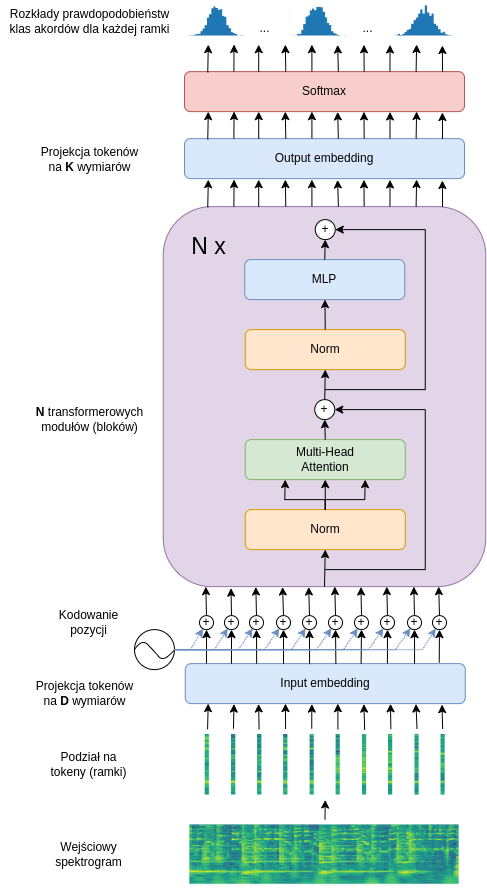
\includegraphics[width=0.8\textwidth]{./images/transformer.png}
    \caption{Schemat modelu transformera do rozpoznawania akordów muzycznych.}
    \label{fig:transformer}
\end{figure}

% ogólny opis architektury - wejście
Rysunek \ref{fig:transformer} prezentuje wykorzystany do treningów model sieci neuronowej --- transformer. Architektura tego modelu jest bardzo prosta. Na wejście sieci podawany jest składający się z $N$ ramek spektrogram $\defmatrix{S}{N}{F}$, który następnie dzielony jest (tylko ideowo, w praktyce to wciąż pojedyncza macierz) na ramki (wektory $\vec s_i \in \mathbb{R}^F$). Ramki odgrywają rolę tokenów, czyli np. kolejnych słów w przypadku przetwarzania języka naturalnego. Transformer przetwarza cały ciąg tokenów równolegle, co jest jego podstawową przewagą nad sieciami rekurencyjnymi, które przetwarzają ciąg tokenów w sposób sekwencyjny. W praktyce jednocześnie przez sieć może przejść kilka ciągów tokenów, czyli cały \emph{batch} sekwencji. Długość sekwencji tokenów jest zupełnie arbitralna, ten sam model może przetwarzać sekwencje różnej długości, zarówno w treningu, jak i później, podczas inferencji.

% ogólny opis architektury - input embedding i positional encodding
W pierwszej kolejności sekwencja ramek (macierz $\matrix{S}$) przechodzi przez pojedynczą warstwę liniową, która rzutuje tokeny wejściowe na wybraną dla danego modelu liczbę wymiarów $d_{\mathrm{model}}$:
\begin{equation}
    \matrix{T_{in}} = \matrix{S} \matrix{W_{in}}
\end{equation}
gdzie $\defmatrix{T_{in}}{N}{d_{\mathrm{model}}}$ to wyjściowa macierz tokenów a $\defmatrix{W_{in}}{F}{d_{\mathrm{model}}}$ to macierz parametrów tej warstwy. Liczba wymiarów $d_{\mathrm{model}}$, podobnie jak liczba tokenów $N$, nie zmienia się podczas przechodzenia przez kolejne warstwy, co różni transformer od sieci splotowych, gdzie rozmiar danych przechodzących przez sieć jest sukcesywnie zmniejszany. W rzeczywistości istnieją architektury oparte o oryginalny transformer, które podobnie jak sieć splotowa, zmniejszają rozmiar danych wejściowych \cite{liu_swin_2021}, ale to tylko głupie wymysły Microsoftu. Przed wejściem do stanowiących właściwą część transformera serii bloków, do tokenów dokładana jest informacja o ich pozycji w sekwencji --- jest to kodowanie pozycji (ang. \emph{positional encoding}). Szczegóły tej operacji zostały opisane poniżej.

% ogólny opis architektury - bloki, w tym MLP i normalizacja
Centralną część transformera stanowi ciąg identycznych bloków BLK. Liczba tych bloków ($B$), w połączeniu z wymiarowością tokenów ($d_{\mathrm{model}}$), stanowią główne hiperparametry modelu i decydują o jego rozmiarze. Każdy blok składa się z dwóch głównych warstw: warstwy atencyjnej MSA (ang. \emph{Mulit-Head Self-Attention}) i niewielkiego perceptronu wielowarstwowego MLP (ang.  \emph{Mulitlayer Perceptron}). Każdą z tych warstw poprzedza normalizacja Norm typu \emph{Layer Normalization} \cite{ba_layer_2016}, a kończy połączenie rezydualne \cite{he_deep_2015}, czyli dodanie do wartości na wyjściu nieznormalizowanej wartości z wejścia. Operacje realizowane przez pojedynczy blok dla ciągu tokenów $\defmatrix{T}{N}{d_{\mathrm{model}}}$ można opisać równaniami:
\begin{eqnarray}
     \textrm{MSA}'(\matrix{T}) = \textrm{MSA}(\textrm{Norm}(\matrix{T})) + \matrix{T} \\
     \textrm{MLP}'(\matrix{T}) = \textrm{MLP}(\textrm{Norm}(\matrix{T})) + \matrix{T} \\
     \textrm{BLK}(\matrix{T}) = \textrm{MLP}'(\textrm{MSA}'(\matrix{T}))
\end{eqnarray}
Zastosowana normalizacja aplikowana jest niezależnie (choć równolegle) dla każdego tokena $t \in \mathbb{R}^{d_{\mathrm{model}}}$ z sekwencji $\matrix{T}$. Polega ona na odjęciu wartości średniej tokena oraz podzieleniu przez jego odchylenie standardowe. Przedstawia to wzór:
\begin{equation}
    \textrm{Norm}(t) = \frac{t - \textrm{E}[t]}{\sqrt \textrm{Var}[t]} \cdot \gamma + \beta
\end{equation}
gdzie $\gamma$ i $\beta$ to trenowane parametry warstwy, przesuwające i skalujące odpowiednio wynik normalizacji. Jeżeli chodzi o perceptron wielowarstwowy, to ma ona zawsze dwie warstwy ukryte, z wymiarem ukrytym czterokrotnie większym niż $d_{\mathrm{model}}$ oraz funkcją aktywacji GELU.
\begin{equation}
    \textrm{MLP}(\matrix{T}) = \textrm{GELU}(\matrix{T}\matrix{W_1} + b_1)\matrix{W_2} + b_2
\end{equation}
gdzie wejściem jest sekwencja tokenów $\defmatrix{T}{N}{d_{\mathrm{model}}}$, macierze $\defmatrix{W_1}{d_{\mathrm{model}}}{4d_{\mathrm{model}}}$, $\defmatrix{W_2}{4d_{\mathrm{model}}}{d_{\mathrm{model}}}$ oraz wektory (dodawane do każdego wiersza odpowiedniej macierzy) $b_1 \in \mathbb{R}^{4d_{\mathrm{model}}}$ i $b_2 \in \mathbb{R}^{d_{\mathrm{model}}}$ to parametry dwóch warstw ukrytych perceptronu wielowarstwowego.

% ogólny opis architetury - dropout
W rzeczywistości pojedynczy blok zawiera jeszcze jeden opcjonalny element, jakim są warstwy \emph{dropout}, umieszczone w trzech miejscach: po funkcji aktywacji w module MLP oraz po każdym z dwóch połączeń rezydualnych, czyli w połowie bloku i na jego wyjściu. Dodatkowo \emph{dropout} może być stosowany również przed wejściem do sieci, czyli bezpośrednio na spektrogramie. Warstwy tego typu zerują z wybranym prawdopodobieństwem niektóre z przechodzących przez nie wartości w celu regularyzacji sieci i uniknięcia przetrenowania. Technika ta jest opcjonalna i nie była stosowana we wszystkich eksperymentach.

% ogólny opis architektury - wyjście (klasyfikacja)
Po serii bloków następuje ostatnia część modelu, odpowiedzialna za klasyfikację. Najpierw, utrzymywana przez wszystkie bloki, wymiarowość tokenów jest zmieniana przez warstwę liniową, w zależności od liczby klas $K$.
\begin{equation}
    \matrix{T_{out}} = \matrix{T} \matrix{W_{out}}
\end{equation}
gdzie $\defmatrix{T_{out}}{N}{K}$ to macierz wyjściowa, $\defmatrix{T}{N}{d_{\mathrm{model}}}$ to macierz sekwencji tokenów a $\defmatrix{W_{out}}{d_{\mathrm{model}}}{K}$ to macierz parametrów tej warstwy liniowej. Następnie dla każdego tokena $t \in \mathbb{R}^K$ zwracany jest rozkład prawdopodobieństwa przynależności do poszczególnych klas akordów, za pomocą funkcji \emph{softmax}:
\begin{equation}
    \textrm{softmax}(t_i) = \frac{\exp{t_i}}{\sum_{j=1}^{K}\exp{t_j}}
\end{equation}
gdzie $t_i$ to $i$-ty element wektora (tokena) $t$. Podsumowując, na wejściu sieci jest spektrogram, składający się z $N$ ramek i $F$ cech, a na wyjściu jest $N$ rozkładów prawdopodobieństwa między $K$ klas, dla każdej z ramek spektrogramu. Wszystkie ramki spektrogramu są więc klasyfikowane jednocześnie, ale z uwzględnieniem kontekstu, jaki tworzą razem.

\subsection{Kodowanie pozycji tokenów}

% positional encoding
Jak widać na rysunku \ref{fig:transformer}, pomiędzy projekcją tokenów wejściowych a wejściem do serii bloków, jest jeszcze etap kodowania pozycji każdego z tokenów. Etap ten jest niezbędny, aby zawrzeć w każdym z tokenów informację o tym, jaka jest jego pozycja w sekwencji. W przypadku sieci rekurencyjnych informacja ta jest zawarta niejawnie, poprzez przetwarzanie tokenów jeden po drugim, w odpowiedniej kolejności. W przypadku transformerów, gdzie tokeny są przetwarzane równolegle, informacja ta musi być dodana jawnie.  Istnieje wiele sposobów, według których można zakodować pozycję tokenów, głównie dzielących się na wykorzystanie wartości wyuczonych (parametry modelu) i stałych (odpowiednia funkcja).  W niniejszej pracy wykorzystane zostało podejście oryginalnych twórców transformera, oparte o wartości funkcji sinus i kosinus. Polega ono na tym, że dla każdego tokena (dla każdej pozycji) generuje się wektor, który ma tę samą liczbę wymiarów co token, dzięki czemu może być do niego dodany. Wartości tych wektorów zdefiniowane są wzorami:
\begin{equation}
    PE_{(\textrm{pos},2i)} = \sin(\textrm{pos}/10000^{2i/d_{\textrm{\tiny model}}})
\end{equation}
\begin{equation}
PE_{(\textrm{pos},2i + 1)} = \cos(\textrm{pos}/10000^{2i/d_{\textrm{\tiny model}}})
\end{equation}
Równania te oznaczają, że każdy wymiar wektora kodującego pozycję odpowiada sinusoidzie o innej częstotliwości. Parzyste pozycje w wektorze to wartości odpowiednich funkcji sinus dla danej pozycji, a nieparzyste to wartości funkcji kosinus dla danej pozycji. Stosowany jest również wariant, gdzie pierwsza połowa wektora to wartości funkcji sinus a druga to wartości funkcji kosinus. Autorzy uzasadniają, że użycie tych funkcji pozwala modelowi łatwo wykorzystywać informację o pozycji, ponieważ między wektorami prezentującymi różne pozycje występują zależności liniowe. Na rysunku \ref{fig:positional_encoding} przedstawiono graficzną reprezentację wektorów kodujących pozycję, dla sekwencji składającej się ze 100 tokenów (wiersze), gdzie liczba wymiarów każdego z nich to 256 (kolumny).
\begin{figure}
    \centering
    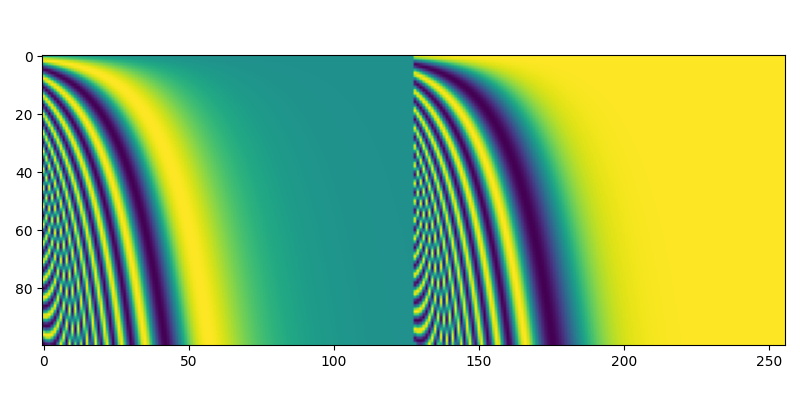
\includegraphics[width=1.0\textwidth]{./images/positional_encoding.png}
    \caption{Przykład wektorów kodujących pozycję dla sekwencji 100 tokenów o wymiarowości 256.}
    \label{fig:positional_encoding}
\end{figure}

\subsection{Multi-Head Self-Attention}

% mutli-head self-attention - wstęp
Najważniejszą część transformera stanowi warstwa atencyjna MSA. Jako jedyna w całym modelu odpowiada ona za ,,wymianę'' informacji między tokenami --- uwzględnienie kontekstu pozostałych tokenów w sekwencji, podczas tworzenia nowej reprezentacji danego tokena.

% mutli-head self-attention - ogólnie o mechaniźmie attention
Sama idea mechanizmu \emph{Attention} polega na tym, że mając dla danego tokena wejściowego zapytanie (ang. \emph{query}) i mając zbiór par klucz-wartość (ang. \emph{key-value}) związanych z innym (lub tym samym) ciągiem tokenów, wylicza się nową reprezentację tokena jako ważoną sumę tych wartości, gdzie wagi są wyliczane na podstawie dopasowania zapytania do kluczy. Wagi te informują więc o tym, jak dużo uwagi powinno poświęcić się danej wartości, tworząc nową reprezentację danego tokena. W przypadku zadania tłumaczenia maszynowego mechanizm ten pozwala skupić się na odpowiednich częściach sekwencji wejściowej, podczas tworzenia sekwencji wyjściowej. Jeżeli zarówno zapytania, jak i pary klucz-wartość pochodzą z tej samej sekwencji tokenów, mamy do czynienia z \emph{Self-Attention}. Warstwa tego typu wyznacza więc dla każdego tokena w sekwencji zapytanie, klucz i wartość, a następnie tworzy jego nową reprezentację jako ważoną sumę wartości pozostałych tokenów. Informacje zakodowane w poszczególnych tokenach mieszają się zatem między sobą. W praktyce warstwa atencyjna w transformerze realizuje równolegle kilka niezależnych operacji \emph{Self-Attention}, których wyniki na końcu są łączone w całość, stąd też nazwa \emph{Multi-Head Self-Attention}. Pozwala to uzyskać lepsze rezultaty niż pojedyncza operacja, nawet jeżeli wykorzysta się niżej wymiarowe reprezentacje.

% mutli-head self-attention - dokładnie jak działa, wzorki
Na wejściu warstwy atencyjnej w transformerze znajduje się macierz $\defmatrix{T}{N}{d_{\mathrm{model}}}$, czyli sekwencja $N$ tokenów. Dla każdego z nich, za pomocą zwykłych warstw liniowych, wylicza się $H$-krotnie trzy wektory: zapytanie $q_i \in \mathbb{R}^{d_k}$, klucz $k_i \in \mathbb{R}^{d_k}$ oraz wartość $v_i \in \mathbb{R}^{d_v}$, gdzie $i \in [1, H]$. Dla całej sekwencji tokenów wektory te tworzą macierze $\defmatrix{Q_i}{N}{d_k}$, $\defmatrix{K_i}{N}{d_k}$ oraz $\defmatrix{V_i}{N}{d_v}$. Przedstawiają to równania:
\begin{eqnarray}
    \matrix{Q_i} = \matrix{T} \matrix{W_i^Q} \\\
    \matrix{K_i} = \matrix{T} \matrix{W_i^K} \\\
    \matrix{V_i} = \matrix{T} \matrix{W_i^V} \\\
\end{eqnarray}
gdzie macierze $\defmatrix{W_i^Q}{d_{\mathrm{model}}}{d_k}$, $\defmatrix{W_i^K}{d_{\mathrm{model}}}{d_k}$ oraz $\defmatrix{W_i^V}{d_{\mathrm{model}}}{d_v}$ to macierze parametrów warstw liniowych tworzących $i$-tą trójkę: zapytanie, klucz i wartość.

Dla pojedynczej trójki macierzy $\matrix{Q}$, $\matrix{K}$ i $\matrix{V}$ operacja \emph{Self-Attention} wygląda następująco:
\begin{equation} \label{eq:sa}
    \textrm{SA}(\matrix{Q}, \matrix{K}, \matrix{V}) = \textrm{softmax}(\frac{\matrix{Q}\matrix{K^T}}{\sqrt{d_k}})\matrix{V}
\end{equation}
Człon ,,$\textrm{softmax}(\frac{\matrix{Q}\matrix{K^T}}{\sqrt{d_k}})$'' oznacza wyliczenie macierzy atencji między wszystkimi parami klucz-zapytanie, poprzez wykonanie iloczynów skalarnych dla każdej z tych par, przeskalowanie uzyskanych wartości i wykorzystanie normalizującej funkcji \emph{softmax}. Dlatego też funkcja SA nazywa się właściwie \emph{Scaled Dot-Product Attention}.  Wartości w uzyskanej macierzy atencji pełnią rolę wag, które następnie są użyte do stworzenia nowej reprezentacji wszystkich tokenów, za pomocą średniej ważonej wektorów z macierzy $\matrix{V}$.  Wynik operacji SA jest więc macierzą, o wymiarach $N \times d_v$.

Cała operacja \emph{Multi-Head Self-Attention} polega na $H$-krotnym wykonaniu operacji \emph{Self-Attention}, których wektory wynikowe są łączone i ostatecznie rzutowane z powrotem na $d_{\mathrm{model}}$ wymiarów. Przedstawiają to poniższe wzory:
\begin{equation}
    \textrm{MSA}(\matrix{T}) = \textrm{Concat}(\textrm{SA}(\matrix{Q_1}, \matrix{K_1}, \matrix{V_1}), ..., \textrm{SA}(\matrix{Q_H},
    \matrix{K_H}, \matrix{V_H}))\matrix{W^O}
\end{equation}
gdzie macierz $\defmatrix{W^O}{Hd_v}{d_{\mathrm{model}}}$ to parametry ostatniej w ramach bloku atencyjnego warstwy liniowej, która rzutuje sklejone wektory z pojedynczych operacji SA na początkowe $d_{\mathrm{model}}$ wymiarów. Dzięki temu wymiarowość tokenów na wyjściu z warstwy atencyjnej pozostaje taka sama jak na wejściu. W niniejszej pracy zastosowane zostało powszechne podejście, aby liczbę wymiarów wektorów zapytań, kluczy i wartości ustalić z góry i uzależnić od liczby wymiarów tokenów i liczby równoległych operacji SA. Zależność ta jest następująca:
\begin{equation}
    d_k = d_v = \frac{d_{\mathrm{model}}}{H}
\end{equation}
Poza wspomnianymi wcześniej hiperparametrami $B$ i $d_{\mathrm{model}}$ istotna dla funkcjonowania modelu jest również liczba $H$ równoległych operacji SA, nazywana również ,,liczbą głów''. Wszystkie hiperparametry transformera zostały zebrane w tabeli \ref{tab:transformer_params}.

\begin{table}
    \centering
    \caption{Hiperparametry transformera.}
    \label{tab:transformer_params}
    \begin{tabular}{|c|l|} \hline
        Symbol & Znaczenie \\ \hline
        $F$ & Wymiarowość na wejściu \\
        $d_{\mathrm{model}}$ & Wymiarowość tokenów wewnątrz sieci \\
        $B$ & Liczba bloków transformera \\
        $H$ & Liczba ,,głów'' w bloku MSA \\
        $K$ & Liczba klas na wyjściu \\
        $p_d$ & Prawdopodobieństwo warstw \emph{dropout} \\ \hline
    \end{tabular}
\end{table}

\subsection{Dwukierunkowy transformer do rozpoznawania akordów --- BTC}

W pracy referencyjnej \cite{park_bi-directional_2019} autorzy postanowili wprowadzić drobne modyfikacje w stosunku do oryginalnego bloku transformera tworząc swój autorski model nazwany \emph{bi-directional transformer for chord recognition} (BTC). Pierwszą z nich jest zamiana warstw liniowych w module MLP, na jednowymiarowe warstwy splotowe z polem recepcyjnym szerokości 3 tokenów.  Według autorów ma to ułatwić sieci tworzenie bardziej ,,wygładzonych'' predykcji i lepsze wykorzystanie kontekstu otaczającego każdą ramkę. Druga różnica polega na tym, że pojedynczy blok transformerowy został rozbity na dwa, które dostają te same wartości na wejściu, a ich wartości wyjściowe są łączone za pomocą dodatkowej warstwy liniowej. Bloki te różnią się operacją MSA.  Została w nich zastosowana technika maskowania, polegająca na modyfikacji macierzy atencji (wzór \ref{eq:sa}) w ten sposób, że dla danego tokena, wagi wszystkich wcześniejszych lub późniejszych tokenów są zerowane. Oznacza to, że tworząc nową reprezentację danego tokena wykorzystuje się jedynie tokeny poprzedzające, lub następujące po nim. W modelu BTC każdy z dwóch bloków tworzących moduł MSA ma inny kierunek maskowania. Technika ta ma zmusić model do pełnego wykorzystywania zarówno wcześniejszego, jak i późniejszego kontekstu przy klasyfikacji danej ramki.



\section{Treningi nadzorowane}

% wstęp
Pierwszy z dwóch rodzajów wykonywanych treningów sieci to klasyczny trening nadzorowany.  Wykorzystywane są w nim dane z oznaczeniami, aby nauczyć model rozwiązywania konkretnego problemu --- klasyfikacji akordów muzycznych. 

% TODO: parę słów o koncepcji treningów nadzorowanych

\subsection{Procedura treningu}

% walidacja krzyżowa, zbiory i epoki
W ramach niniejszej pracy, do oceny jakości modeli wykorzystana została pięciokrotna walidacja krzyżowa. Oznacza to, że pojedynczy eksperyment, związany z pojedynczym zestawem hiperparametrów modelu, zbioru danych i treningu, składa się z pięciu treningów. W każdym z nich jedna z pięciu części zbioru danych wykorzystana jest do walidacji, a pozostałe cztery do nauki. Możliwe jest, aby ograniczyć cały zbiór danych do wybranych zbiorów oznaczeń, co zupełnie nie zmienia zasady działania walidacji krzyżowej, ponieważ w ramach każdego zbioru oznaczeń zachowany jest podział na pięć równych części. Treningi dzieli się na epoki, które z definicji oznaczają pojedyncze przejście przez wszystkie dostępne dane treningowe (w tym przypadku cztery z pięciu części zbioru). Jak opisano w rozdziale \ref{sec:preprocessing}, w przypadku przeprowadzonych eksperymentów, pojedyncza epoka oznacza kilkukrotne przejście przez wszystkie utwory treningowe, ale dla każdego utworu przetwarzany jest jedynie jego losowy fragment (lub fragmenty).

% kroki
Na epokę składają się kroki, gdzie każdy krok oznacza jedną zmianę parametrów modelu. W ramach każdego kroku model przetwarza równolegle cały \emph{batch} 10-sekundowych fragmentów utworów.  Ponieważ, ze względów optymalizacyjnych, na jeden przykład ze zbioru danych składa się kilka fragmentów tego samego utworu, to na realny rozmiar batcha wpływają dwa parametry: liczba analizowanych równolegle przykładów (czyli utworów) oraz liczba zwracanych jednocześnie fragmentów pojedynczego utworu. Dla każdej ramki, z każdego fragmentu wejściowego, model zwraca predykcję akordów, w postaci rozkładów prawdopodobieństw. Rozkłady te są następnie porównywane z rzeczywistymi klasami akordów za pomocą funkcji kosztu, jaką jest entropia krzyżowa (ang. \emph{cross-entropy}). Dla pojedynczej ramki, czyli dla pojedynczego wyjściowego rozkładu prawdopodobieństw $t \in \mathbb{R}^K$ i indeksu $k$, oznaczającego numer rzeczywistej klasy tej ramki, entropia krzyżowa ma postać:
\begin{equation}
    \textrm{CE}(t, k) = - \log t_k
\end{equation}
Wartość tę uśrednia się później między wszystkimi tokenami (ramkami) i między sekwencjami (fragmentami), aby uzyskać pojedynczą liczbę rzeczywistą, reprezentującą błąd popełniany przez sieć.  Następnie, zgodnie z algorytmem \emph{backpropagation}, obliczane są pochodne cząstkowe (gradient) tej funkcji kosztu po wszystkich parametrach modelu. Do optymalizacji parametrów modelu na podstawie obliczonych pochodnych wykorzystany jest algorytm optymalizacyjny \emph{AdamW}. Współczynnik nauki (ang. \emph{learning rate}), przez pierwszych pięć epok ma jedynie dziesiątą część swojej docelowej wartości, aby zapewnić małe zmiany parametrów modelu na początku treningu. Transformery są bowiem podatne na to, że z powodu zbyt dużych kroków w początkowej fazie treningu, przestaną zbiegać do konkretnego rozwiązania. Co więcej, na potrzeby późniejszej analizy, w każdym kroku zapisywane są wartości funkcji kosztu i metryki \emph{accuracy} dla obecnego batcha przykładów.

\subsection{Walidacja i wczesne zatrzymanie treningu}

% walidacja i wczesne zatrzymanie
Pod koniec każdej epoki, po przejściu przez całą część treningową (cztery z pięciu części), następuje bieżąca ocena modelu na części walidacyjnej (ostatnia z pięciu części). Celem tego etapu jest zobaczyć, jak model radzi sobie z przykładami, na których nie był uczony. Można w ten sposób rozpoznać moment, kiedy sieć zaczyna się przetrenowywać i zatrzymać trening (ang. \emph{early stopping}). Aby zapewnić stabilność wyników tej oceny, nie stosuje się w niej, tego samego co podczas nauki, mechanizmu losowania fragmentów utworów. Nie stosuje się również augmentacji. Zamiast tego, dla każdego utworu wykonuje się po kolei predykcję klas dla wszystkich ramek. Szczegóły procedury predykcji klas akordów dla całego utworu zostały opisane poniżej. Mając dla danego utworu predykcję wszystkich akordów, oblicza się na tej podstawie wartość metryki \emph{accuracy}. Po przejściu przez całą część walidacyjną, wyniki te agregowane są do pojedynczej wartości. Podczas przechodzenia przez kolejne epoki, zapamiętywana jest najlepsza wartości \emph{accuracy}, wraz z numerem danej epoki i aktualnym stanem modelu. Jeżeli wartość \emph{accuracy} nie wzrasta przez zadaną liczbę epok, trening zostaje wstrzymany.

\subsection{Ewaluacja modelu}

% ewaluacja
Po wstrzymaniu treningu z powodu przetrenowania modelu lub po przejściu przez zadaną liczbę epok, model zostaje przywrócony do stanu, dającego najlepsze wyniki na części walidacyjnej. Następnie na tejże części wykonywana jest bardziej dogłębna ocena wytrenowanej sieci. Polega ona, podobnie jak podczas treningu, na wytworzeniu predykcji, na podstawie których, dla każdego utworu wyliczane są dodatkowo: 
\begin{itemize}
    \item ciąg wystąpień akordów (\code{ChordOccurence}), o określonym czasie rozpoczęcia i
        zakończenia w sekundach (ciąg takich samych predykcji jest łączony w jedno wystąpienie
        akordu)
    \item wartość miary CSR (ang. \emph{Chord Symbol Recall}) na podstawie
        ciągu wystąpień akordów, która ma postać
        \begin{displaymath}
            \textrm{CSR} = \frac
                        {\textrm{całkowity czas trwania poprawnie zaklasyfikowanych fragmentów}}
                        {\textrm{całkowity czas trwania utworów}}
        \end{displaymath}
    \item wartości miar klasyfikacyjnych, liczonych tak, że pojedyncza ramka jest traktowana, jak
        pojedyncza predykcja:
        \begin{itemize}
            \item dokładność (ang. \emph{accuracy}; $1$ wartość)
            \item czułość (ang. \emph{recall}) per klasa ($25$ wartości)
            \item precyzja (ang. \emph{precision}) per klasa ($25$ wartości)
            \item macierz pomyłek (ang. \emph{confusion matrix})
        \end{itemize}
\end{itemize}
Ciąg wystąpień akordów zapisywany jest w pliku \filetype{lab}, a wartości metryk CSR, dokładności, czułości, precyzji i macierz pomyłek w pliku \filetype{json}. Dodatkowo macierz pomyłek zapisywana jest jako obrazek w pliku \filetype{png}. Następnie wartości wszystkich tych miar są agregowane dla całego zbioru i również zapisywane w plikach \filetype{json} i \filetype{png}. Jeżeli chodzi o wartości miary CSR, to aby zagregować ją dla wszystkich utworów liczy się średnią ważoną, gdzie wagą jest długość trwania utworu --- miara ta nazywa się wtedy WCSR (ang. \emph{Weighted Chord Symboll Recall}). Co do zapisywanej na obrazku ,,globalnej'' macierzy pomyłek, to jest ona normalizowana wierszami, czyli wartości na głównej przekątnej są równoważne czułości modelu dla danej klasy. Implementacja całej procedury ewaluacji modelu znajduje się w pliku \url{src/training/evaluate.py}.

% problem podwójnego wykorzystania zbioru walidacyjnego + uzasadnienie wykorzystania walidacji krzyżowej
Jak można zauważyć, część walidacyjna jest w pojedynczym treningu wykorzystywana na dwa sprzeczne sposoby. Po pierwsze służy do oceny jakości modelu na koniec procesu nauki. Jest to więc typowe zastosowanie, zgodne z zasadami walidacji krzyżowej. Z drugiej jednak strony, ten sam zbiór jest wykorzystywany do wykrycia przetrenowania i wczesnego zatrzymania treningu. Prowadzi to do swego rodzaju ,,przetrenowania'' pod część walidacyjną, ponieważ wybierany jest ten stan modelu, który wiadomo, że daje najlepsze wyniki dla danych przykładów. W takich sytuacjach, kiedy nie stosuje się walidacji krzyżowej, standardowo dzieli się zbiór na trzy części: treningową do nauki, testową do ostatecznej oceny i walidacyjną do oceny podczas treningu i uniknięcia przetrenowania. Technikę tę --- dzielenie zbioru na trzy części --- można zastosować również dla walidacji krzyżowej, jeżeli jest to konieczne. W przypadku tej pracy zostało to jednak uznana za zbędne, z tego powodu, że właściwym celem oceny modeli jest porównanie ich między sobą, a nie poznanie jak najlepszego przybliżenia ich rzeczywistej dokładności (rola zupełnie odrębnego zbioru testowego). Fakt, że każdy z nich daje nieznacznie zawyżone wyniki na części walidacyjnej, nie utrudnia porównania ich między sobą. Najważniejsze jest to, że walidacja krzyżowa pozwala uniknąć problemu obciążenia pojedynczego, niewielkiego zbioru testowego. Obciążenie takie, charakterystyczne dla zbyt małego, niereprezentatywnego zbioru, uniemożliwia rzetelne porównanie modeli między sobą. Łatwo może wtedy bowiem dojść do sytuacji, kiedy model wydaje się lepszy od innych, bo przypadkowo daje lepsze wyniki na małym zbiorze testowym, choć dla przykładów spoza tego zbioru radzi sobie znacznie gorzej.

\subsection{Implementacja i wykorzystana infrastruktura}

% implementacja i sprzęt
Pętla treningowa została zaimplementowana w pliku \url{src/training/training.py}. Została ona przygotowana w taki sposób, aby można było trenować modele w sposób rozproszony, zgodnie z techniką \emph{Distributed Data Parallel}. Do rejestrowania treningów, ich hiperparametrów i wartości metryk wykorzystano system \emph{MLflow}\footnote{\url{https://mlflow.org/}}. Treningi odbywały się na jednej lub kilku kartach graficznych NVIDIA GeForce RTX 3090.

\subsection{Podsumowanie parametrów treningu}

% podsumowanie parametrów treningu
Wszystkie ustawienia pojedynczej serii pięciu treningów (eksperymentu), włączając w to parametry zbioru danych, hiperparametry modelu i hiperparametry samej pętli treningowej, zostały przedstawione w tabeli \ref{tab:sup_training_params}. Wartości parametrów z tej tabeli są wymieniane dla każdego udokumentowanego eksperymentu. W rzeczywistości przygotowana implementacja umożliwia również zmianę parametrów, które zostały wybrane jako niezmienne dla niniejszej pracy i opisane w rozdziale \ref{sec:preprocessing}, takich jak długość przetwarzanego przez model fragmentu (100 ramek). Te parametry nie zostały wymienione w tabeli, ponieważ nie różnią się między eksperymentami. Pominięte również zostały parametry o charakterze ściśle technicznym, takie jak wykorzystanie pamięci podręcznej w RAM-ie, czy wykorzystanie treningu rozproszonego.

% wszystkie parametry wynikające z argparse (F-fixed, T-technical, X-changed between experiments)
% DATASET
% F   sample_rate=22050
% F   frame_size=2048
% F   hop_size=2048
% F   frames_per_item=100
% X   item_multiplier
% X   song_multiplier
% F   audio_preprocessing (cqt, raw)=CQT
% F   standardize_audio=YES
% X   pitch_shift_augment
% F   labels_vocabulary=MAJ_MIN
% X   subsets
% X   dataset_fraction (TODO: opisać w rozdziale o datasecie)
% T   use_ram_cache
% MODEL
% X   model_dim
% X   n_heads
% X   n_blocks
% X   block_type
% X   dropout_p
% T   extra_features_dim=NO
% T   pretrained_encoder_path
% T   pretrained_encoder_run_name
% TRAINING
% T   experiment_name
% T   run_name
% X   n_epochs
% X   batch_size
% X   lr
% X   early_stopping
% T   ddp
% T   num_workers

\begin{table}
    \centering
    \caption{Hiperparametry pojedynczego treningu nadzorowanego.}
    \label{tab:sup_training_params}
    \begin{tabular}{|l|p{0.6\linewidth}|} \hline
        \multicolumn{2}{|c|}{ZBIÓR DANYCH} \\ \hline
        \code{item\_mutliplier} & Liczba przykładów zwracanych dla jednego utworu \\
        \code{song\_multiplier} & Liczba przejść przez wszystkie utwory w jednej epoce \\
        \code{augment} & Czy zastosowano augmentacje \\
        \code{subsets} & Jakie podzbiory zostały wykorzystane do treningu \\
        \code{fraction} & Jaka część zbioru treningowego została wykorzystana do treningu \\ \hline
        \multicolumn{2}{|c|}{MODEL} \\ \hline
        \code{model\_dim} & Liczba wymiarów pojedynczego tokena przechodzącego przez model \\
        \code{n\_heads} & Liczba równoległych operacji MSA \\
        \code{n\_blocks} & Liczba bloków w modelu \\
        \code{block\_type} & Typ bloku: BTC lub zwykły transformer \\
        \code{dropout\_p} & Prawdopodobieństwo zerowania w warstwach \emph{dropout} \\ \hline
        \multicolumn{2}{|c|}{TRENING} \\ \hline
        \code{n\_epochs} & Liczba epok w treningu \\
        \code{batch\_size} & Liczba utworów przetwarzanych w jednym kroku \\
        \code{lr} & Współczynnik uczenia \\
        \code{early\_stopping} & Maksymalna liczba epok bez wzrostu dokładności na części walidacyjnej \\ \hline
    \end{tabular}
\end{table}

\subsection{Zasady predykcji akordów dla całego utworu}

Najprostszym sposobem, aby uzyskać predykcję dla całego utworu, który zazwyczaj składa się z kilku tysięcy ramek, jest podanie wszystkich ramek jednocześnie na wejście sieci neuronowej. O ile transformer może teoretycznie przyjąć na wejściu sekwencję dowolnej długości (ograniczeniem jest oczywiście pamięć), to w przypadku sekwencji dłuższych niż w treningu, wymaga to od modelu pewnej generalizacji. Jest to więc podejście ryzykowne i mało praktyczne, ze względu na ograniczenie pamięci, które w praktyce może spowodować, że i tak będzie trzeba dzielić utwór na kilka części.

Najbezpieczniej podawać więc na wejście modelu fragmenty takiej długości jak w treningu, czyli po $100$ ramek na raz. Pozostaje zdecydować, czy fragmenty mają się na siebie nakładać i jeśli tak, to w jaki sposób agregować kilka możliwych predykcji dla jednej ramki. W niniejszej pracy zdecydowano się na takie podejście, zgodnie z którym z każdej $100$-elementowej sekwencji, jedynie środkowe $50$ branych jest do ostatecznego wyniku. Pozostałe $25$ ramek z początku i $25$ ramek z końca traktowane są jako kontekst. Wynika to z niezweryfikowanej hipotezy, że predykcje dla ramek z szerszym kontekstem przed nimi i po nich, są precyzyjniejsze, niż dla ramek na brzegu fragmentu, dla których nie wiadomo dobrze, co działo się przed nimi lub po nich. Oznacza to w praktyce, że kolejne fragmenty nakładają się na siebie w połowie. 

Cała procedura wytwarzania predykcji dla pojedynczego nagrania polega więc na:
\begin{itemize}
    \item podzieleniu nagrania na rozłączne fragmenty po $50$ ramek
    \item dodaniu do każdego fragmentu po $25$ ramek z fragmentów wcześniejszego i późniejszego, w
        przypadku pierwszego i ostatniego fragmentu, uzupełnić powtórzoną wielokrotnie odpowiednio
        pierwszą i ostatnią ramką
    \item wykonaniu predykcji dla wszystkich utworzonych w ten sposób fragmentów, po $100$ ramek
        każdy
    \item wyciągnięciu $50$ środkowych akordów z każdej sekwencji wyjściowej i złączeniu ich w jedną
        sekwencję, o długości równej liczbie ramek utworu
\end{itemize}
Mechanizm ten, w ogólnej postaci, zaimplementowany został w funkcji \code{partial\_predict} w pliku \url{src/training/evaluate.py}. W rzeczywistości, wszystkie nakładające się na siebie fragmenty, są przetwarzane przez model równolegle, jako jeden batch przykładów.

Proporcja między długością pojedynczego fragmentu ($100$ ramek) a długością kontekstu (po $25$ ramek przed i po), została ustalona na podstawie intuicji. Nie przeprowadzono żadnej dokładnej analizy ani eksperymentów, aby ustalić, jaki ma ona wpływ na jakość predykcji. Możliwe jest zarówno to, że bez nakładania na siebie fragmentów, predykcje nie byłyby w ogóle (lub znacząco) gorsze, jak i to, że zwiększenie długości kontekstu, poprawiłoby istotnie predykcje sieci.



\section{Samonadzorowane treningi wstępne}

% wstęp - co to self-supervised - ogólna koncepcja (TODO: czy to tutaj czy nie?)
Nienadzorowany, a dokładnie samonadzorowany (ang. \emph{self-supervised}) trening wstępny, stanowi kluczową część niniejszej pracy. Algorytmy tego typu polegają na wykonywaniu przez sieć specjalnego, dodatkowego zadania pomocniczego (ang. \emph{pretext task}), w wyniku którego model uczy się ekstrahować wysokopoziomowe, abstrakcyjne, bogate semantycznie cechy. Treningi takie zbudowane są dokładnie tak samo jak treningi nadzorowane, ale samo zadanie (wraz z oznaczeniami) jest wytworzone sztucznie i nie wymaga oznaczeń przygotowanych przez człowieka. Przykładem może być układanie przez sieć neuronową puzzli \cite{noroozi_unsupervised_2017}, dorysowywanie brakującego fragmentu rysunku \cite{pathak_context_2016}, czy też uzupełnianie słów w zdaniach \cite{devlin_bert_2019}. Algorytmów tych jest bardzo wiele i można podzielić je na wiele różnych rodzajów, które wykorzystywane są dla różnych typów danych (czasami kilku jednocześnie \cite{jia_scaling_2021}). Ze względu na ogromną dostępność danych nieoznaczonych (Internet), metody tego typu zyskują bardzo na popularności w ostatnich latach. W dziedzinach przetwarzania języka naturalnego i rozpoznawania mowy są już właściwie standardem. Wytrenowany za pomocą takich metod model, może być później dotrenowany (ang. \emph{finetuning}) w sposób nadzorowany, na zbiorze danych związanym z konkretnym zadaniem. Jeżeli trening wstępny się udał, może przynieść on różnego rodzaju zysk dla zadania docelowego, w porównaniu do treningu od zera. Przykładami są:
\begin{itemize}
    \item krótszy wymagany czas treningu nadzorowanego
    \item mniejszy wymagany zbiór danych oznaczonych
    \item mniejsza podatność na przetrenowanie
    \item lepsza generalizacja i w ogóle lepsza ostateczna jakość modelu
\end{itemize}

% wstęp - jaki zastosowano algorytm - ogólna idea, że na podstawie MAE, BERT, wav2vec
Zastosowany w ramach niniejszej pracy algorytm uczenia samonadzorowanego, stanowi autorską adaptację algorytmu MAE (ang. \emph{Masked Auto-Encoders}) \cite{he_masked_2021}, pochodzącego z obszaru przetwarzania obrazów. Algorytm MAE ma naturę bardzo ogólną i sam jest właściwie adaptacją oryginalnego algorytmu BERT \cite{devlin_bert_2019}, stosowanego w dziedzinie przetwarzania języka naturalnego. Bardzo podobnym rozwiązaniem z dziedziny rozpoznawania mowy jest również \cite{baevski_wav2vec_2020}. Wszystkie te rozwiązania opierają się na tej samej, bardzo prostej koncepcji: maskowaniu (wycinaniu) fragmentu danych wejściowych (obrazka, zdania, nagrania) i uczeniu sieci uzupełniania tych danych. Aby poprawnie uzupełnić brakujące fragmenty, model musi nauczyć się interpretować i ,,rozumieć'' pozostałą, widoczną część danych wejściowych. Zaproponowana adaptacja tychże algorytmów dla nagrań muzycznych, co do zasady, polega więc na maskowaniu fragmentów spektrogramu wejściowego i uczeniu modelu uzupełniania tychże, wyciętych fragmentów.

\subsection{Architektura autoenkodera uzupełniającego fragmenty spektrogramu}

% opis modelu - propozycja uproszczona
Do uzupełniania zamaskowanych fragmentów spektrogramu wykorzystany jest nieznacznie bardziej skomplikowany model niż stosowany w treningach nadzorowanych. W praktyce można oczywiście wykorzystać do tego celu czysty transformer. Maskowanie polegałoby wtedy na wypełnieniu części tokenów wejściowych jakąś stałą wartością. Na wyjściu sieci trzeba by oczekiwać, poprzez przyłożenie odpowiedniej funkcji kosztu, że na pozycjach zamaskowanych tokenów model wydedukuje rzeczywiste, oryginalne wartości tychże tokenów, sprzed operacji maskowania. Podejście to, choć proste, niesie za sobą pewne konsekwencje, jak potrzeba przetwarzania wielu takich samych, zamaskowanych tokenów, czy też poświęcenie części modelu (końcowych warstw) na realizację zadania zamiany abstrakcyjnej reprezentacji danych na format spektrogramu. W praktyce ważne jest bowiem jedynie to, aby uzyskać dobry ekstraktor cech, a nie zrealizować jak najlepiej samo zadanie wstępne.

\begin{figure}
    \centering
    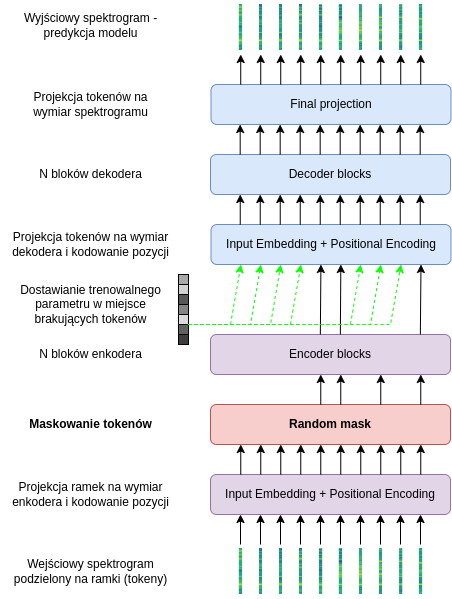
\includegraphics[width=0.8\textwidth]{./images/mae_transformer.png}
    \caption{Schemat autoenkodera uzupełniającego fragmenty spektrogramu.}
    \label{fig:mae_transformer}
\end{figure}

% opis modelu - dokładny opis na podstawie rysunku
Idąc za pomysłem twórców algorytmu MAE, zastosowana została architektura składająca się z dwóch części --- enkodera i dekodera --- które razem tworzą autoenkoder. Każdy z nich jest po prostu osobnym transformerem, ale dekoder powinien być zdecydowanie mniejszy. Cały model zaprezentowany jest na rysunku \ref{fig:mae_transformer}. Na wejściu do modelu znajduje się spektrogram. Następnie, zgodnie z opisaną już wcześniej zasadą działania transformera, ramki są rzutowane na odpowiednią dla enkodera liczbę wymiarów i dodawane jest do nich kodowanie pozycji. Następuje później kluczowa operacja maskowania, która odbywa się na poziomie sekwencji tokenów. Polega ona na usunięciu losowej części sekwencji, zgodnie z odpowiednimi, opisanymi poniżej założeniami. Enkoder przetwarza następnie jedynie niezamaskowane tokeny, dzięki czemu dla dużych proporcji maskowania zmniejsza się znacząco złożoność wymaganych obliczeń. Jest to jeden z głównych atutów wspomnianego algorytmu MAE. Po przejściu przez wszystkie bloki eknodera niezamaskowana część sekwencji powinna być docelowo przedstawiana w postaci wektorów bogatych semantycznie cech. Przed wejściem do dekodera, skrócona sekwencja jest z powrotem rozszerzana do oryginalnej długości. Wykorzystuje się w tym celu specjalny, trenowalny wektor odpowiedniej długości, który jest wstawiany w miejsce wszystkich zamaskowanych tokenów. Cała sekwencja przechodzi później przez dekoder, którego zadaniem jest wytworzyć spektrogram, jak najbardziej zbliżony do oryginalnego. Aby to zrobić, musi uzupełnić zamaskowane tokeny na podstawie informacji, jaką w niezamaskowanej części sekwencji umieścił enkoder. Mały rozmiar dekodera wymusza wyciągnięcie jak najwięcej informacji z widocznych tokenów przez enkoder. Co więcej, ponieważ dekoder przetwarza już pełną sekwencję tokenów, to jego rozmiar wpływa bardzo na złożoność obliczeń.

\subsection{Zasady maskowania spektrogramów}

% maskowanie spektrogramów - wstęp
Operacja maskowania spektrogramów, jak już wspomniano, odbywa się na poziomie całej sekwencji --- maskowane są zawsze całe tokeny, a nie ich fragmenty. Jest to oczywiście jedno z możliwych podejść, można bowiem próbować maskować również fragmenty tokenów. Zastosowane podejście pozwala jednak bardzo łatwo na optymalizację, polegającą na przetwarzaniu przez enkoder jedynie niezamaskowanej części sekwencji.

% maskowanie spektrogramów - kwestia proporcji
Indeksy wycinanych tokenów są losowane, a proporcja między ich liczbą a liczbą pozostawionych tokenów jest hiperparametrem danego treningu samonadzorowanego. W przypadku maskowania słów w zdaniach \cite{devlin_bert_2019} wycinana jest jedynie niewielka część ($15\%$) sekwencji, ponieważ każdy pojedynczy token (słowo), ma już w sobie bardzo dużo informacji --- bardzo bogate i szerokie, abstrakcyjne znaczenie. W przypadku maskowania obrazów \cite{he_masked_2021} jest dokładnie odwrotnie --- wycinana jest spora część obrazu ($75\%$), ponieważ pojedyncze piksele mają w sobie niewiele informacji i mogą być skutecznie uzupełnione przez zwykłą interpolację liniową. W przypadku spektrogramów sytuacja jest bardziej zbliżona do obrazów, ponieważ uzupełnienie pojedynczych ramek również można zrealizować poprzez nieskomplikowaną interpolację. Co więcej, charakter spektrogramów dla utworów muzycznych jest taki, że często ich długie, trwające ułamek sekundy lub nawet kilka sekund fragmenty są stałe. Zależy to oczywiście od gatunku i od tego, które fragmenty spektrogramu są brane pod uwagę. Jeżeli chodzi natomiast o częstość zmian akordów w zachodniej muzyce popularnej, to w $10$-sekundowych fragmentach będą się one często zmieniać zaledwie kilka razy. Z tego powodu, aby zadanie uzupełniania spektrogramów było dość wymagające, maskowana część musi najprawdopodobniej zajmować przynajmniej kilkadziesiąt procent długości całej sekwencji.

% maskowanie spektrogramów - kwestia wielkości dziur
Poza proporcją maskowania, istotne jest również to, czy wycinane ramki będą tworzyły dłuższe, ciągłe fragmenty. Wynika to z faktu, że uzupełnienie co drugiej ramki, choć proporcja maskowania wynosi $50\%$, wciąż pozostaje stosunkowo łatwym zadaniem. Natomiast uzupełnienie trwającego $2$ sekundy ciągłego fragmentu, chociaż jest to tylko piąta część całej sekwencji, stanowi zadanie znacznie trudniejsze i wymaga głębszej interpretacji widocznych fragmentów nagrania. Dlatego też drugim hiperparametrem treningu samonadzorowanego jest liczba ciągłych bloków, na które dzielona jest cała sekwencja. Kiedy następuje operacja maskowania, tokeny są wycinane lub pozostawiane jedynie w ciągłych grupach, tworzących te bloki. Za pomocą tego parametru i proporcji maskowania można modyfikować trudność zadania między samonadzorowanymi treningami wstępnymi.

% maskowanie spektrogramów - łatwa implementacja
Omawiając zasady maskowania spektrogramów, warto wspomnieć o jeszcze jednej zalecie tego algorytmu --- jest on bardzo łatwy w implementacji. Maskowanie można zrealizować jako wykonanie permutacji sekwencji tokenów i odcięcie odpowiedniej ich liczby. Aby po przejściu przez bloki enkodera uzyskać sekwencję oryginalnej długości i kolejności, wystarczy dokleić odpowiednią liczbę razy wektor oznaczający zamaskowane tokeny i wykonać permutację odwrotną. Podejście to można stosować również wtedy, kiedy chce się zachować zadaną liczbę ciągłych bloków w ramach sekwencji.

\subsection{Procedura treningu}

% eksperymenty, treningi, zbiory i epoki
W przypadku treningów samonadzorowanych, na pojedynczy eksperyment składa się tylko jeden trening, ponieważ nie stosowano tutaj metod takich jak walidacja krzyżowa. Sama nauka odbywa się na podstawie wszystkich danych nieoznaczonych ($10000$ utworów), które tworzą zbiór treningowy. Dane te, pomijając fakt, że nie mają oznaczeń, przetwarzane są do postaci $10$-sekundowych spektrogramów dokładnie w taki sam sposób, jak w treningach nadzorowanych. Stosowane są również te same augmentacje. We wszystkich wykonanych eksperymentach nienadzorowanych wykorzystany jest pełny zbiór treningowy. Mimo braku oznaczeń wciąż konieczne jest jednak aby sprawdzać, czy zbiór nie uczy się danych treningowych na pamięć. W tym celu pierwsza z pięciu części danych oznaczonych (same nagrania, bez augmentacji) wykorzystana jest jako zbiór walidacyjny. Dokładnie tak jak w eksperymentach nadzorowanych, trening dzieli się na epoki, gdzie pojedyncza epoka oznacza kilkukrotnie przejście przez wszystkie nagrania treningowe, ale dla każdego z nich losowany jest zawsze jeden $10$-sekundowy fragment.

% kroki, maskowanie, predykcja i funkcja kosztu
Epoki dzielą się na kroki, gdzie każdy krok to równoległe przetworzenie całego batcha $10$-sekundowych fragmentów i jednokrotna modyfikacja parametrów modelu. W ramach danego kroku generowana jest pojedyncza maska (lista numerów tokenów), stosowana dla wszystkich fragmentów w batchu. Dla pojedynczej ramki wyjściowej $f' \in \mathbb{R}^F$ i pojedynczej ramki wejściowej $f \in \mathbb{R}^F$, wyliczany jest błąd średniokwadratowy (ang. \emph{mean squared error}) pełniący rolę funkcji kosztu, zgodnie ze wzorem:
\begin{equation}
    \textrm{MSE} = \frac{1}{F} \sum_{i=1}^{F} (f'_{i} - f_{i})^2
\end{equation}
Wartość ta jest wyliczana tylko dla tych ramek, które były zamaskowane (wycięte) i uśredniana między nimi, oraz między sekwencjami. Ma to zmusić model do skupienia się na zadaniu rekonstrukcji, a nie kopiowaniu wartości wejściowych.  Następnie, w standardowy sposób, parametry całego autoenkodera są optymalizowane na podstawie gradientu błędu średniokwadratowego.  Wartość funkcji kosztu jest logowana dla każdego batcha.

% walidacja
Po przejściu przez wszystkie przykłady treningowe z epoki następuje etap bieżącej walidacji modelu, mający na celu uniknięcie przetrenowania. Dokładnie tak samo jak dla danych uczących, wyliczane są predykcje na fragmentach ze zbioru walidacyjnego i obliczana jest wartość tej samej funkcji kosztu.  Wartość ta jest logowana i służy jedynie porównaniu z wartością na zbiorze treningowym --- nie wylicza się na jej podstawie pochodnej i nie optymalizuje parametrów modelu. W przeciwieństwie do treningów nadzorowanych, zbiór walidacyjny jest przetwarzany tak samo jak zbiór treningowy, poprzez losowanie $10$-sekundowych fragmentów dla kolejnych utworów. Podejście to jest zdecydowanie wystarczające aby ocenić, czy model zaczyna się uczyć na pamięć.

% po walidacji
Na koniec każdej epoki, stan enkodera jest zapisywany, aby umożliwić późniejsze wykorzystanie go do rozpoznawania akordów (treningów nadzorowanych). Dodatkowo aby ułatwić ocenę stanu autoenkodera, która jest dość trudna na podstawie samej wartości błędu średnikowadratowego, wybierane są trzy losowe przykłady ze zbioru walidacyjnego. Każdy z nich zapisywany jest w postaci obrazka z trzema spektrogramami: wejściowy z przed operacji maskowania, zamaskowany przed wejściem do sieci i predykcja sieci. Ocena konkretnych predykcji modelu pozwala ocenić na ile rzeczywiście model nauczył się rozumieć strukturę nagrań muzycznych.

\subsection{Implementacja i wykorzystana infrastruktura}

% implementacja i sprzęt
Cała procedura treningu samonadzorowanego wraz konstrukcją autoenkodera została zaimplementowana w pliku \url{src/training/mae_training.py}. Podobnie jak trening nadzorowany, przygotowana zostala możliwość treningu rozproszonego, a wszystkie hiperparametry i metryki są logowane do systemu \emph{MLflow}. Treningi odbywały się na jednej lub kilku kartach graficznych NVIDIA GeForce RTX 3090.

\subsection{Podsumowanie parametrów treningu}

% podsumowanie parametrów treningu
Wszystkie ustawienia pojedynczego treningu samonadzorowanego, włączając w to parametry zbioru danych i hiperparametry autoenkodera zostały przedstawione w tabeli \ref{tab:mae_training_params}.  Wartości parametrów z tej tabeli są wymieniane dla każdego udokumentowanego eksperymentu. Tak samo jak dla treningów nadzorowanych, pominięte zostały niektóre stałe lub techniczne ustawienia, opisane w poprzednich rozdziałach. 

% wszystkie parametry wynikające z argparse (F-fixed, T-technical, X-changed between experiments)
% DATASET
% F   sample_rate=22050
% F   frame_size=2048
% F   hop_size=2048
% F   frames_per_item=100
% X   item_multiplier
% X   song_multiplier
% F   audio_preprocessing (cqt, raw)=CQT
% F   standardize_audio=YES
% X   pitch_shift_augment
% F   labels_vocabulary=MAJ_MIN
% T   subsets=None
% F   dataset_fraction=1.0
% T   use_ram_cache
% ENKODER
% X   encoder_dim
% X   encoder_n_heads
% X   encoder_n_blocks
% T   encoder_extra_features_dim=NO
% T   pretrained_encoder_path
% T   pretrained_encoder_run_name
% DEKODER
% X   decoder_dim
% X   decoder_n_heads
% X   decoder_n_blocks
% TRENING
% X   masking_ration
% X   chunks_per_item
% T   experiment_name
% T   run_name
% X   n_epochs
% X   batch_size
% X   lr
% T   ddp

\begin{table}
    \centering
    \caption{Hiperparametry pojedynczego samonadzorowanego treningu wstępnego.}
    \label{tab:mae_training_params}
    \begin{tabular}{|l|p{0.6\linewidth}|}
        \hline \multicolumn{2}{|c|}{ZBIÓR DANYCH} \\ \hline
        \code{item\_mutliplier} & Liczba przykładów zwracanych dla jednego utworu \\
        \code{song\_multiplier} & Liczba przejść przez wszystkie utwory w jednej epoce \\
        \code{augment} & Czy zastosowano augmentacje \\
        \hline \multicolumn{2}{|c|}{ENKODER} \\ \hline
        \code{encoder\_dim} & Liczba wymiarów pojedynczego tokena przechodzącego przez enkoder \\
        \code{encoder\_n\_heads} & Liczba równoległych operacji MSA w enkoderze\\
        \code{encoder\_n\_blocks} & Liczba bloków w enkoderze \\
        \hline \multicolumn{2}{|c|}{DEKODER} \\ \hline
        \code{decoder\_dim} & Liczba wymiarów pojedynczego tokena przechodzącego przez dekoder \\
        \code{decoder\_n\_heads} & Liczba równoległych operacji MSA w dekoderze\\
        \code{decoder\_n\_blocks} & Liczba bloków w dekoderze \\
        \hline \multicolumn{2}{|c|}{TRENING} \\ \hline
        \code{masking\_ratio} & Proporcja maskowania --- jaka część sekwencji tokenów jest wycinana \\
        \code{chunks\_per\_item} & Liczba ciągłych, niepodzielnych bloków w sekwencji \\
        \code{n\_epochs} & Liczba epok w treningu \\
        \code{batch\_size} & Liczba utworów przetwarzanych w jednym kroku \\
        \code{lr} & Współczynnik uczenia \\ \hline
    \end{tabular}
\end{table}
